\section{抽象语法树AST}
\label{AST}
AST是MiniC采用的第一重中间表示,它由在词法/语法分析阶段生成。由于我们在AST上完成了符号表的生成和类型检查,因此这两部分也在本章介绍。
\subsection{生成}
\label{genAST}
AST的结构是根据上下文无关文法的产生式定义的:一个终结符节点是一棵AST;一棵以产生式左部非终结符为根的AST的子节点按从左到右顺序分别是其右部分法符号所产生的AST。

比如有如下产生式:
\begin{displaymath}
	A:=aBcD
\end{displaymath}
其中大写字母代表非终结符,小写字母代表终结符,那么以非终结符A为根的AST就是如下形式:
\dirtree{%
.1 A.
.2 a.
.2 以非终结符B为根的AST.
.2 c.
.2 以非终结符D为根的AST.
}
注意到AST的定义实际上也给出了其产生方法:只要在做LR分析时,随着规约的进行,将子树与根进行连接即可。

在实现时,AST的叶节点在词法分析时生成,内部节点在语法分析时在不同的产生式的语法规则指导下生成,并在规约时连接到其父节点上。

下面给出一个MiniC的AST节点所包含的内容:
\label{ASTnode}
\begin{lstlisting}
typedef struct AST_NODE{
  	int nodeType;//节点类型,即节点代表了哪个文法符号
  	int nodeLevel;//节点深度
	union node_content content; //节点包含的内容,只有叶子节点才不为空,在词法分析时添加
  	AST_NODE * father;//父节点
  	AST_NODE * leftChild;//最左子节点
  	AST_NODE * rightSibling;//右兄弟节点

	struct symtbl_hdr* symtbl;//文法符号所在范围的符号表
	AST_NODE* double_list;
}AST_NODE;
\end{lstlisting}
{\it \anchor 有关节点类型的详细定义,请参阅:\verb|AST.h|}\\
{\it \anchor 有关建立AST树的相应过程,请参阅:\verb|AST_operation.c|, \verb|minic.y|}\\
\subsection{生成的语法树示例}
我们利用\verb|dot|生成了下面代码的AST:
\begin{lstlisting}
int main()
{
	int i;
	i = i + 1;
}

\end{lstlisting}

\begin{center}
	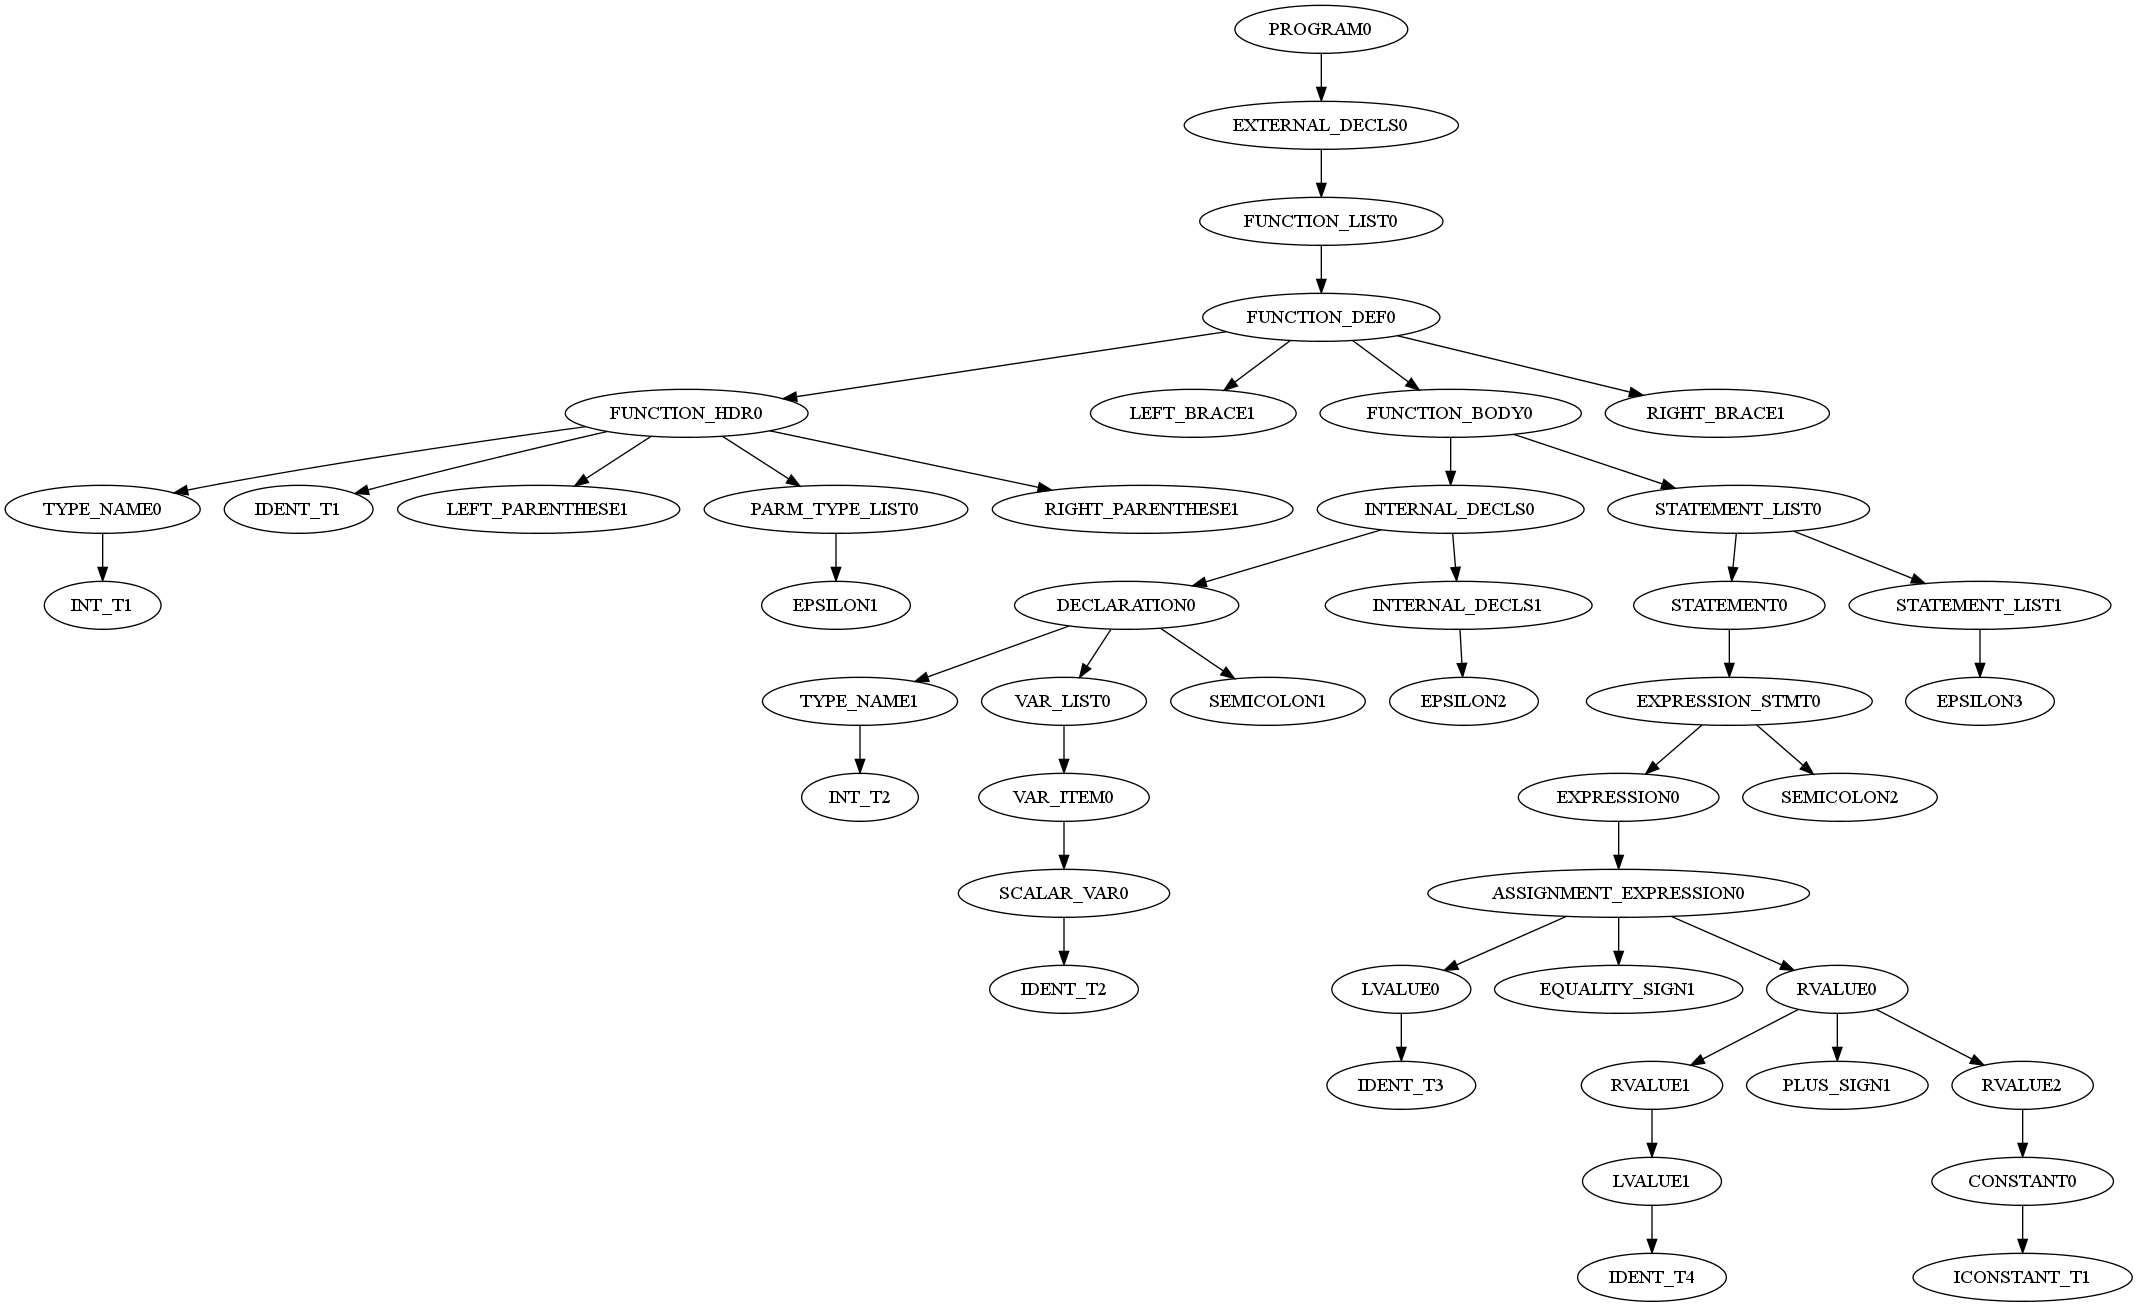
\includegraphics[scale=0.2]{grammer_tree.png}
	\captionof{figure}{AST示例}
	\label{fig:grammertree}
\end{center}
{\it \manerrarrow MiniC的验证工具中提供了两种方式查看输入源文件的语法树:\verb|dot|和ASCII ART,请参阅MiniC使用手册}\\
\subsection{AST的通用周游模板}
\label{ASTtravesal}
由于建立符号表、类型检查以及将AST变换成三元式都涉及到在AST上做深度游先周游,所以我们设计了一个通用的周游函数\verb|tree_traversal|,该函数接受两个参数:AST的根节点指针以及返回值为\verb|int|,参数为AST节点指针的函数指针的数组。由于我们将所有的节点类型都定义成了不同的整数,因此只需要为不同的周游阶段构造不同的函数指针数组,在\verb|tree_traversal|中周游到某个节点时以节点类型为数组下标定位到对这个节点进行操作的函数并调用,就能够用同一个深度游先周游函数完成不同的周游功能。\\
{\it \anchor 有关深度优先周游模板的代码,请参阅:\verb|symtbl_operation.h|}\\

\subsection{符号表}
\label{symtbl}
符号表对于一个编译程序而言是最为重要的一个部分,从它创建以后开始的每一个步骤中,“标识符”(函数名、变量名)的出现,就意味着要在符号表中找到对应的表项,提取要使用的信息。

\paragraph*{符号表的结构}
符号表的层次结构需要根据语言的特性来决定。例如在MiniC中,由于存在着全局变量、函数声明、语句块等特点,因此符号表需要组织成树状结构。

符号表的具体底层数据结构可以有很多种选择,常见的有哈希表、链表和线性表,在MiniC中,由于考虑到输入源文件的规模都较小,所以采用可扩张的线性表来实现\footnote{这种线性表在空间不足时会另外申请一块两倍的空间并拷贝自己}。在这种实现下,插入一个表项的均摊开销是$O(1)$,检索一个表项的开销是$O(n)$,$n$为表项总数目。


MiniC的符号表结构如下:
\begin{enumerate}
\item 每个作用域(函数、复合语句)一张符号表:
\begin{lstlisting}
struct symtbl_hdr
{
	symtbl_hdr* parent_tbl; //父表
	symtbl_hdr* leftChild_tbl; //最左子表
	symtbl_hdr* rightSibling_tbl;	//右兄弟子表

	//ret_type, ret_star, para_num, func are useful only for function's symtbl
	char* func_name; //函数名,若该表属于复合语句则该项为空
	int ret_type; //函数返回值基类型
	int ret_star; //函数返回值是否为指针类型
	int para_num; //该函数的参数个数
	int func_def; //该函数是否有定义
	int item_num; //符号表表项数目
	int maxSize; //全部表项占用的内存大小,字节
	symtbl_item* item; //表项列表
}
\end{lstlisting}
\item 每张符号表都有一个表项列表:
\begin{lstlisting}
struct symtbl_item
{
	int isGlobal; //是否为全局变量
	int type; //表项的基类型
	int star_num; //表项是否为指针
	int writable; //表项是否为只读类型
	char* name; //符号名 
	int size; //数组大小,非数组为0
	int func_off; //
	int offset; //在内存分配中的偏移
};

\end{lstlisting}
\end{enumerate}
注意到在一个函数的符号表中,函数的参数和它的局部变量是存放在一起的,这种将参数和局部变量视作同类的安排能够为以后的内存分配、寄存器分配等提供一些方便。



\paragraph*{在AST上生成符号表}
如前所述,AST上包含了源文件中所有的信息,因此只需要扫描AST的某些子树,提取符号名称、类型、作用域等信息,就可以生成符号表。

具体的做法是:先序深度优先周游AST,找到作用域入口(\verb|FUNCTION_DEF|和\verb|COMPOUND_STMT|)并将当前作用于压入作用域栈,然后在该作用域节点下寻找类型为\verb|EXTERNAL_DECLS|和\verb|INTERNAL_DECLS|的节点,分情况处理该节点的函数和变量的声明,将名称和类型(包括函数的返回类型,参数、参数类型)加入符号表,作用域从作用域栈顶取得。在作用域出口(周游函数返回时)弹出作用域栈顶。\\
{\it \anchor 有关符号表生成的相关代码,请参阅:\verb|gen_symtbl.h|}\\

\paragraph*{在符号表上查询符号}
由于符号表是树状组织,因此查询时要从给定的一张符号表开始,在表中查找,如果未找到符号,就在当前表的父表中查找,直到找到该符号或者在最高级的\verb|Global Scope|也没有找到返回空。
\\
{\it \anchor 有关符号表查询的代码,请参阅:\verb|symtbl_operation.h|}\\
\paragraph*{符号表生成与语义检查}
\label{declchk}
在符号表生成的过程中,实际上还要进行一项语义检查:同一作用域的多重定义问题。即在向当前符号表中添加符号时,如果该符号已经出现在了当前表中,就要报告错误,停止建立符号表。

\subsection{符号表示例}
下图展示了以下代码的符号表:
\begin{lstlisting}
int i,j;
void f(int k)
{
	int i,j;
}
int main()
{
	int i,j;
	{int k;}
}
\end{lstlisting}
\begin{center}
	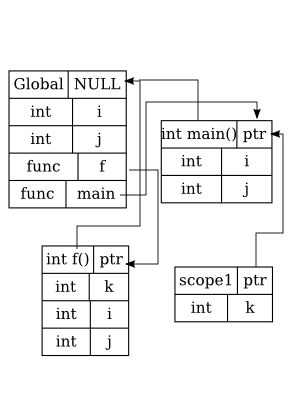
\includegraphics[scale=0.6]{symtbl.png}
	\captionof{figure}{符号表示例}
	\label{symtbl}
\end{center}
{\it \manerrarrow MiniC的验证工具中提供了查看源文件生成的符号表的方法:请参阅MiniC使用手册}\\
\subsection{类型检查}
\label{typeveri}
类型检查是语义检查的一部分,这一步骤的主要目的是排除所有符合语法但不符合运算规则、函数调用规则的语句。类型检查的对象是表达式语句,这包括:
\begin{itemize}
	\item 检查一元、二元运算符作用的对象;报告类型无效的运算对象
	\item 检查传入函数的实参类型和函数的参数表对应形参的类型是否兼容;报告兼容性警告或者错误
	\item 检查赋值语句两边类型是否是赋值兼容的(包括检查函数返回值);报告兼容性警告或者错误
\end{itemize}
类型检查一旦完成,表明这份源代码已经能够且必须通过后续的变换,直到生成目标代码。
\paragraph*{类型检查的规则} 下面的表格给出了MiniC类型检查的所有规则以及应对方法。
%TODO: 类型检查规则表
\paragraph*{在AST上做类型检查}
类似于生成符号表,类型检查同样要对AST进行深度优先周游,在发现\verb|STATMENT|类型的节点时开始按照不同的语句类型以及语句中不同的元素类型开始进行类型检查。


\section{三元式}
\label{triple}
三元式是MiniC的第二重中间表示。同MiniC源文件中复杂的语句和操作相比,三元式相对简单、只有少数指令并且更接近目标代码表示。

MiniC中,一条三元式可以表示为如下形式:
\begin{itemize}
\item A: 一般的运算指令:\verb|(i): op arg1, arg2|, \verb|arg|可以是\verb|(j)|也可以是标识符或立即数;\verb|arg2|若无效则为单元操作
\item B: 条件跳转指令:\verb|(i): if arg goto (j)|,\verb|arg|可以是\verb|(j)|也可以是标识符或立即数
\item C: 无条件跳转指令:\verb|(i): goto (j)|
\item D: 传参指令:\verb|(i): param arg|,\verb|arg|可以是\verb|(j)|也可以是标识符或立即数;出现在调用指令前
\item E: 调用指令:\verb|(i): call (j)|
\item F: 作用域指令:\verb|(i): enter|, \verb|(i): leave|用于指示作用域的变化
\item G: 布尔专用指令:\verb|(i): setrb|, \verb|(i): getrb|用于组合布尔表达式的翻译,后面会有详细叙述
\end{itemize}
\subsection{三元式的结构}
\label{triplestruct}
考虑到后续在三元式上的操作,三元式并不以上述的字符串的形式储存,以结构的形式存在一个可扩张的线性表中(类似于符号表的实现)。下面给出表项的结构:
\begin{lstlisting}
typedef struct triple
{
	enum operator op;
	union arg arg1;
	union arg arg2;
	int result_type; //运算结果的类型
	int arg1_type; //参量的类型
	int arg2_type; 
	symtbl_hdr* symtbl; //本条三元式所属范围的符号表
	struct basic_block *block; //本条三元式所属的基本块
	int arg1_uni; //在数据流分析时arg1所代表的变量的index
	int arg2_uni; //在数据流分析时arg2所代表的变量的index
	int tmp_uni; //在数据流分析是本条三元式运算结果代表的变量的index
	int label; //本条三元式的标号(仅当本条三元式是跳转语句的目标时有效)
}triple;
\end{lstlisting}

\subsection{三元式指令列表}
\label{tripleinst}
下面的表格给出了MiniC的三元式中所有的\verb|op|以及对应的功能和三元式类型(每种类型的具体解释见本节起始处的说明):
\begin{center}
\begin{minipage}{0.48\textwidth}
\begin{flushleft}
	\begin{tabular}{|l|l|l|}
	\hline
		\verb|op| & 类型 & 功能 \\
	\hline
		\verb|if| & B & 条件成立就跳转 \\
	\hline
		\verb|if_not| & B & 条件不成立就跳转 \\
	\hline
		\verb|goto| & C & 无条件跳转\\
	\hline 
		\verb|negative| & A & 取相反数\\
	\hline
		\verb|not| & A & 取布尔非\\
	\hline
		\verb|address| & A & 取地址\\
	\hline
		\verb|star| & A & 取地址处存放的数据\\
	\hline
		\verb|positive| & A & 返回操作数本身\\
	\hline
		\verb|assign| & A & 值赋给\verb|arg1|\\
	\hline
		\verb|star_assigh| & A & 赋值给地址\\
	\hline 
		\verb|add| & A & 加法\\
	\hline 
		\verb|minus| & A & 减法\\
	\hline
		\verb|multiply| & A & 乘法\\
	\hline 
		\verb|char_to_int| & A & 类型转换\\
	\hline
		\verb|equal| & A & 判断相等\\
	\hline
		\verb|less| & A & 判断是否小于\\
	\hline 
		\verb|larger| & A & 判断是否大于\\
	\hline
		\verb|eqlarger| & A & 判断是否大于等于\\
	\hline
	\end{tabular} 
\end{flushleft}
\end{minipage}
\begin{minipage}{0.48\textwidth}
\begin{flushright}
\begin{tabular}{|l|l|l|}
	\hline
		\verb|op| & 类型 & 功能 \\
	\hline
		\verb|eqless| & A & 判读是否小于等于\\
	\hline 
		\verb|noteq| & A & 判读是否不等于\\
	\hline 
		\verb|or| & A & 布尔或\\
	\hline 
		\verb|and| & A & 布尔与\\
	\hline 
		\verb|setrb| & G & 将\verb|rb|置为\verb|arg|的值\\
	\hline 
		\verb|getrb| & G & 获取\verb|rb|的值\\
	\hline 
		\verb|call| & E & 调用函数\\
	\hline 
		\verb|param| & D & 传参\\
	\hline 
		\verb|enterF| & F & 进入函数\\
	\hline 
		\verb|enterS| & F & 进入复合语句\\
	\hline 
		\verb|leaveF| & F & 离开函数\\
	\hline 
		\verb|leaveS| & F & 离开复合语句\\
	\hline 
		\verb|return| & A & 返回\\
	\hline
		\verb|adds| & A & 左移两位后加\\
	\hline
		\verb|minuss| & A & 左移两位后减\\
	\hline 
		\verb|r_shift| & A & 右移两位\\
	\hline 
		\verb|c_str| & A & 表示一个字符串\\
	\hline
		\verb|Imm| & A & 表示一个大于511的立即数\\
	\hline
	\end{tabular}
	\label{tab:}
\end{flushright}
\end{minipage}
	\captionof{table}{MiniC三元式\lstinline|op|定义}
\end{center}
\subsection{将AST转换为三元式}
这一工作仍然使用\hyperref[ASTtravesal]{AST的通用周游模板}进行,只是操作的对象换成了不同类型的语句(\verb|STATEMENT|)。有关一些特殊语句,例如\verb|for, while, if|的翻译,由于使用的方法同\cite{sunjiasu}的第8章对应部分相似,本文档不再赘述。下面仅介绍转化工作的最困难的部分。
\paragraph*{表达式的转换}
\label{ASTtotriple}
\subsection{生成基本块}
\label{basicblock}
基本块,是一些机器无关的全局优化的操作对象,其定义见\cite{sunjiasu}的第9章。实际实现时,基本块的基本成员仅有几个指针,分别指向块首和块尾以及该块连出和连入的其它基本块。其余的成员都是为了保存数据流分析的结果而设的:
\begin{enumerate}
	
\end{enumerate}

{\it \anchor 有关基本块的完整结构的定义以及基本块的生成函数,请参阅:\verb|basic_block.h, gen_basic_block.c|}\\
\paragraph*{基本块示例}
{\it \manerrarrow MiniC的验证工具中提供了生成基本块图形表示的dot文件的方法,请参阅MiniC使用手册}\\
对于以下的一个函数,它的基本块如下图所示:
\begin{lstlisting}
int main()
{
	int i;
	char p[10];
	for(i = 0 ; i < 10 ; i++){
		p[i] = 'z' - i;
	}
}
\end{lstlisting}
\section{机器无关优化}
\label{indepopt}
%TODO:

